\documentclass[11pt]{article}

% Change "review" to "final" to generate the final (sometimes called camera-ready) version.
% Change to "preprint" to generate a non-anonymous version with page numbers.
\usepackage{acl}
% \usepackage[review]{acl}


% Standard package includes
\usepackage{times}
\usepackage{latexsym}

% For proper rendering and hyphenation of words containing Latin characters (including in bib files)
\usepackage[T1]{fontenc}
% For Vietnamese characters
% \usepackage[T5]{fontenc}
% See https://www.latex-project.org/help/documentation/encguide.pdf for other character sets

% This assumes your files are encoded as UTF8
\usepackage[utf8]{inputenc}

% This is not strictly necessary, and may be commented out,
% but it will improve the layout of the manuscript,
% and will typically save some space.
\usepackage{microtype}

% For mathematics environments like align
\usepackage{amsmath}
\usepackage{amssymb}

% For professional table formatting
\usepackage{booktabs}

% This is also not strictly necessary, and may be commented out.
% However, it will improve the aesthetics of text in
% the typewriter font.
\usepackage{inconsolata}

%Including images in your LaTeX document requires adding
%additional package(s)
\usepackage{graphicx}

% If the title and author information does not fit in the area allocated, uncomment the following
%
%\setlength\titlebox{<dim>}
%
% and set <dim> to something 5cm or larger.

\title{Identifying and Steering Program Validity Awareness Latent Directions in LLMs: A Sparse Autoencoder Analysis of Code Hallucinations}

% Author information can be set in various styles:
% For several authors from the same institution:
% \author{Author 1 \and ... \and Author n \\
%         Address line \\ ... \\ Address line}
% if the names do not fit well on one line use
%         Author 1 \\ {\bf Author 2} \\ ... \\ {\bf Author n} \\
% For authors from different institutions:
% \author{Author 1 \\ Address line \\  ... \\ Address line
%         \And  ... \And
%         Author n \\ Address line \\ ... \\ Address line}
% To start a separate ``row'' of authors use \AND, as in
% \author{Author 1 \\ Address line \\  ... \\ Address line
%         \AND
%         Author 2 \\ Address line \\ ... \\ Address line \And
%         Author 3 \\ Address line \\ ... \\ Address line}

\author{Kriz Royce A. Tahimic \\
  Department of Software Technology\\
  College of Computer Studies\\
  De La Salle University \\
  \texttt{kriz\_tahimic@dlsu.edu.ph}}

%\author{
%  \textbf{First Author\textsuperscript{1}},
%  \textbf{Second Author\textsuperscript{1,2}},
%  \textbf{Third T. Author\textsuperscript{1}},
%  \textbf{Fourth Author\textsuperscript{1}},
%\\
%  \textbf{Fifth Author\textsuperscript{1,2}},
%  \textbf{Sixth Author\textsuperscript{1}},
%  \textbf{Seventh Author\textsuperscript{1}},
%  \textbf{Eighth Author \textsuperscript{1,2,3,4}},
%\\
%  \textbf{Ninth Author\textsuperscript{1}},
%  \textbf{Tenth Author\textsuperscript{1}},
%  \textbf{Eleventh E. Author\textsuperscript{1,2,3,4,5}},
%  \textbf{Twelfth Author\textsuperscript{1}},
%\\
%  \textbf{Thirteenth Author\textsuperscript{3}},
%  \textbf{Fourteenth F. Author\textsuperscript{2,4}},
%  \textbf{Fifteenth Author\textsuperscript{1}},
%  \textbf{Sixteenth Author\textsuperscript{1}},
%\\
%  \textbf{Seventeenth S. Author\textsuperscript{4,5}},
%  \textbf{Eighteenth Author\textsuperscript{3,4}},
%  \textbf{Nineteenth N. Author\textsuperscript{2,5}},
%  \textbf{Twentieth Author\textsuperscript{1}}
%\\
%\\
%  \textsuperscript{1}Affiliation 1,
%  \textsuperscript{2}Affiliation 2,
%  \textsuperscript{3}Affiliation 3,
%  \textsuperscript{4}Affiliation 4,
%  \textsuperscript{5}Affiliation 5
%\\
%  \small{
%    \textbf{Correspondence:} \href{mailto:email@domain}{email@domain}
%  }
%}

\begin{document}
\maketitle
\begin{abstract}
Large Language Models (LLMs) generate code with varying degrees of accuracy, and recent studies have identified hallucinations in over 2,000 instances across 3,000 code samples, indicating substantial room for improvement. Yet, approximately 30\% of AI-suggested code is being integrated into production systems. Despite the risk and wide adoption, the mechanisms by which these models generate between valid and invalid codes remain poorly understood. Hence, we will mechanistically examine how LLMs internally represent their \textit{program validity awareness} through a three-component methodology: (1) dataset building using MBPP (Mostly Basic Python Problems) dataset paired with Gemma 2 2B generated solutions, (2) Sparse Autoencoder analysis using Gemma Scope to identify latent directions corresponding to program validity awareness, and (3) validation through both statistical methods and causal experiments. Our statistical validation employs AUROC and F1 scores, while causal evidence comes from model steering experiments. By analyzing residual stream activations at the final token position, we expect to identify specific latent dimensions that discriminate between correct and incorrect code implementations. This research advances the understanding of code generation mechanisms while offering practical implications for enhancing software development reliability, potentially reducing economic costs of code hallucinations, and improving safety in high-risk domains.
\end{abstract}

\section{Introduction}

The integration of Large Language Models (LLMs) into software development has sparked a fundamental shift in how code is written and maintained across the industry. A comprehensive study by \citet{dohmke2023sea} revealed out of nearly one million developers, approximately 30\% of all AI-suggested code from GitHub Copilot is accepted and integrated into production systems. The same paper also projected that these productivity enhancements could contribute significantly to economic growth, potentially boosting global GDP by over USD 1.5 trillion by 2030 as these technologies help meet the growing worldwide demand for software development.

However, the widespread adoption of code-capable LLMs brings critical concerns regarding their reliability and safety. These concerns are validated by compelling research from \citet{liu2024exploring}, which documented a troubling prevalence of hallucinations—identifying 2,119 instances across just 3,084 code samples. What makes these findings particularly alarming is the fundamental difference between hallucinations in code versus natural language. Unlike hallucinations in natural language generation, which might result in incorrect but plausible text, code hallucinations can produce non-functional, insecure, or potentially harmful implementations. Code hallucinations become particularly concerning in high-risk domains such as healthcare, banking, and the military, where code reliability is paramount.

Despite the widespread adoption and associated risks, the internal mechanisms of these models remain poorly understood, operating largely as black boxes. This challenge has led researchers to explore various interpretability methods to understand and improve these models. Among these approaches, Mechanistic Interpretability has emerged as a promising direction, focusing on revealing how models represent and process information internally. This approach is especially valuable because it helps identify why models make certain mistakes or errors. The insights gained from mechanistic interpretability can inform better architectural choices for neural networks, making it particularly impactful for safety-critical applications.

In their pursuit to mechanistically understand neural networks, researchers discovered a critical challenge: superposition. This phenomenon reveals that neural networks can encode more features than they have available neurons, which might have been the cause of polysemantic neurons. To untangle these overlapping features, researchers turned to Sparse Autoencoders (SAE), which have proven effective at separating these intertwined features into more interpretable components.

After deciding to use SAE to disentangle polysemantic features, researchers face the crucial task of labeling and understanding each latent direction. Some researchers, like \citet{bricken2023monosemanticity} and \citet{templeton2024scaling}, employ a top-down approach that uses a larger LLM to generate labels for each latent direction based on tokens they activate strongly. In contrast, this paper follows what \citet{ferrando2024know} implements, which is a more bottom-up approach that starts with a label or behavior of interest. Their methodology begins with constructing a dataset to elicit a specific latent direction, which will be inputted into the model. The model's internals will then be observed to identify what latent directions activate in response to the feature-specific dataset. 

\citet{ferrando2024know} study uncovered specific latent directions in the model's representation space that encode the model's ability to recognize entities. Using datasets spanning various entity types, including people, movies, cities, and songs, the researchers identified distinct latent directions - some that activate specifically for entities the model can recall facts about and others that activate for entities the model doesn't recognize. Through model steering of these entity recognition latent directions, they demonstrated causal effects on model behavior, showing they could influence whether models would refuse to answer questions about known entities or generate hallucinated information about unknown ones. Their analysis revealed these entity recognition latent directions emerged in the middle layers of the network and regulated how attention mechanisms extracted factual information, providing crucial insights into how models determine whether to generate information or refuse to answer.

While these approaches have successfully revealed latent directions in natural language generation, the application of Sparse Autoencoders to understand program validity awareness latent directions in code-capable LLMs remains unexplored. This represents a significant opportunity to advance our understanding of how models internally represent program validity awareness — the model's self-knowledge if it will generate correct code or not — a critical aspect for improving the reliability and safety of AI-assisted software development.

\section{Methodology}
\label{sec:methodology}

\begin{figure}[!ht]
    \centering
    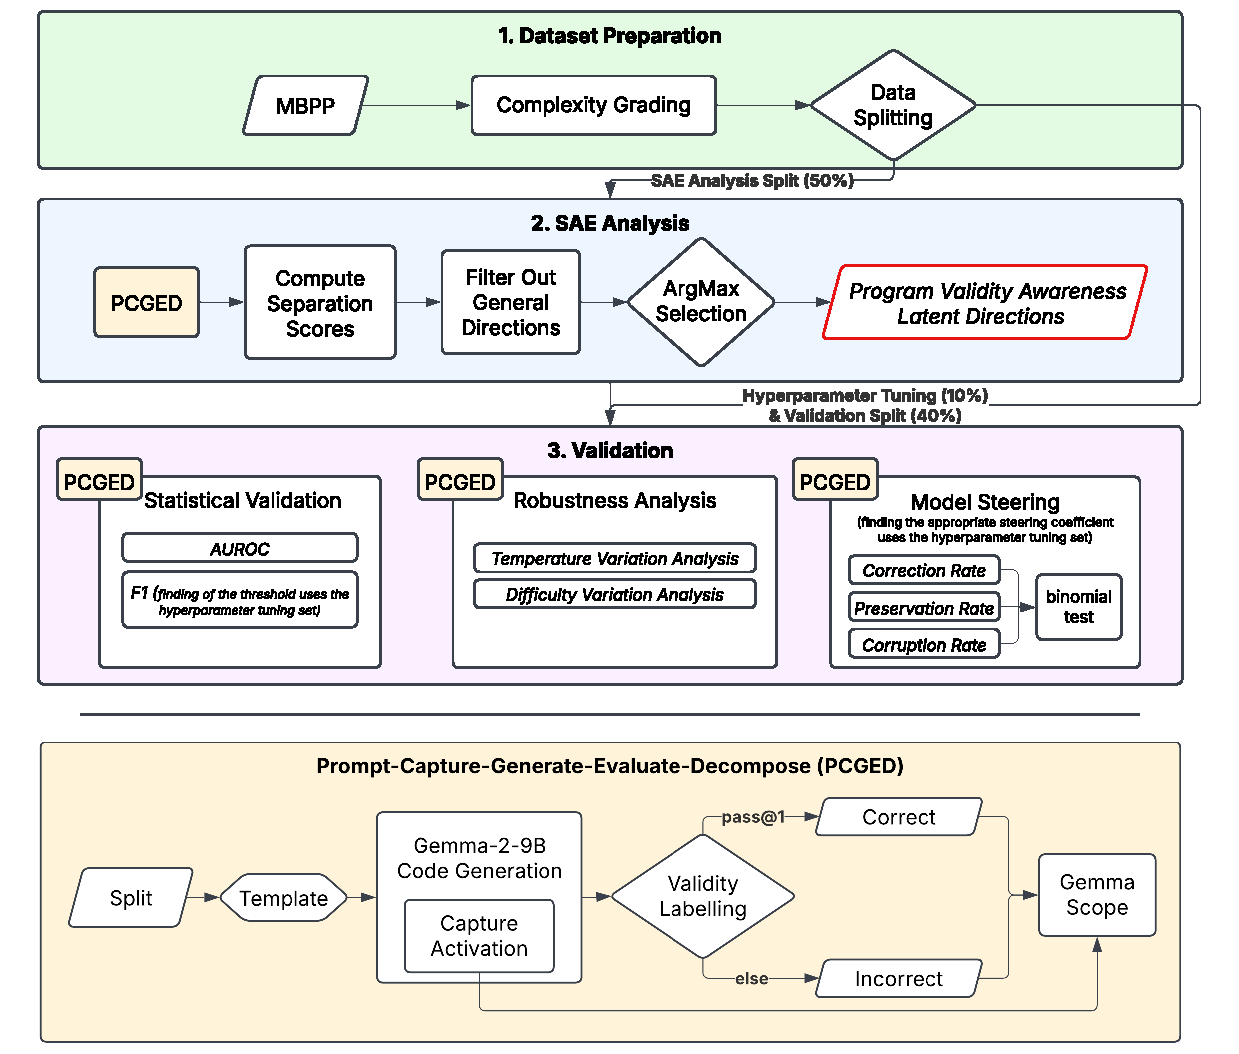
\includegraphics[width=0.99\linewidth]{figures/methodology.pdf}
    \caption{Overview of the three-component methodology: dataset building, SAE analysis, and validation}
    \label{fig:methodology}
\end{figure}

% Adapts
This chapter outlines the methodological approach used in our study, drawing significant inspiration from the work of \citet{ferrando2024know} in their investigation of entity recognition latent in language models. We adapt their framework while introducing key modifications to address our distinct research objectives.

% Three main parts
Our methodology consists of three main components: dataset building to collect and categorize program solutions, SAE activation analysis to identify latent direction, and validation to verify the found program validity awareness latent direction, as illustrated in Figure~\ref{fig:methodology}.

\subsection{Dataset Preparation}

This research utilizes the MBPP (Mostly Basic Python Problems) dataset, which consists of 1,000 Python programming problems designed to evaluate fundamental programming competencies. We enhance the original MBPP dataset by adding a cyclomatic complexity column using McCabe's cyclomatic complexity metric \citep{mccabe1976complexity} to enable complexity-based analysis.

Cyclomatic complexity quantifies the structural complexity of program code by measuring the number of linearly independent paths through the program's control flow graph. The metric is computed using the formula:

\begin{equation}
M = E - N + 2P
\end{equation}

where $M$ represents the cyclomatic complexity, $E$ denotes the number of edges in the control flow graph, $N$ indicates the number of nodes in the graph, and $P$ represents the number of connected components. In the control flow graph representation, nodes correspond to the smallest executable code segments, while directed edges connect these segments based on the program's execution flow. This mathematical foundation allows us to systematically categorize programming problems based on their algorithmic complexity, enabling stratified analysis of how program validity awareness varies across different complexity levels.

The enhanced dataset undergoes stratified random sampling for data splitting to ensure fair representation across complexity levels:

\begin{itemize}
    \item \textbf{Stratification}: Problems are divided into complexity strata using equal-width bins based on complexity scores
    \item \textbf{Randomization}: Task IDs are shuffled within each complexity stratum to ensure fair sampling
    \item \textbf{Interleaving}: A round-robin pattern is applied across all strata simultaneously to prevent complexity bias
\end{itemize}

This approach results in three balanced sets: SAE analysis (50\%), hyperparameter tuning (10\%), and validation (40\%) that maintain proportional complexity distribution. The hyperparameter tuning set is used to optimize classification thresholds for F1 score calculation and determine appropriate steering coefficients for model interventions. 

\subsection{SAE Analysis}

To analyze program validity awareness latent direction in language models, we employ a systematic approach using the PCGED pipeline (detailed in Section~\ref{sec:pcged}) to generate labeled code samples with corresponding model activations. The captured activations are then processed through pre-trained Sparse Autoencoders (SAEs) from GemmaScope \citep{lieberum2024gemma}, which project model representations into higher-dimensional interpretable spaces. The technical architecture of these SAEs is described in the Decompose stage of the PCGED pipeline. This section focuses on our analytical methodology for identifying latent directions that demonstrate program validity awareness.

\subsubsection{Separation Score Analysis}

We analyze the residual stream at the final token for each code sample in our dataset to capture the model's representation during the input phase when the model consumes the programming problem prompt. 

We compute activation statistics for each latent dimension across correct and incorrect code samples. For a given layer $l$ and latent dimension $j$, we calculate the fraction of activations on correct and incorrect code, respectively:

\begin{align}
    f_{l,j}^{\text{correct}} = \frac{\sum_{i}^{N^{\text{correct}}} \mathbf{1}[a_{l,j}(\mathbf{x}_{l,i}^{\text{correct}}) > 0]}{N^{\text{correct}}}, \\  
    f_{l,j}^{\text{incorrect}} = \frac{\sum_{i}^{N^{\text{incorrect}}} \mathbf{1} [a_{l,j}(\mathbf{x}_{l,i}^{\text{incorrect}}) > 0]}{N^{\text{incorrect}}}
\end{align}

To identify latent dimensions that effectively distinguish between correct and incorrect code, we compute separation scores:

\begin{align}
    s_{l,j}^{\text{correct}} = f_{l,j}^{\text{correct}} - f_{l,j}^{\text{incorrect}}, \\
    s_{l,j}^{\text{incorrect}} = f_{l,j}^{\text{incorrect}} - f_{l,j}^{\text{correct}}
\end{align}

\subsubsection{General Language Filtering}

To isolate Python-specific validity features from general language patterns, we apply a filtering step using the pile-10k dataset\footnote{\url{https://huggingface.co/datasets/NeelNanda/pile-10k}}, the first 10,000 samples from the Pile \citep{gao2020pile}. We process these diverse text samples through the same SAE pipeline, extracting activations at random word positions. For each SAE feature, we compute its activation frequency on general text:

\begin{equation}
f_{l,j}^{\text{pile}} = \frac{\sum_{i=1}^{N^{\text{pile}}} \mathbf{1}[a_{l,j}(\mathbf{x}_{l,i}^{\text{pile}}) > 0]}{N^{\text{pile}}}
\end{equation}

Features with $f_{l,j}^{\text{pile}} > 0.02$ are excluded as they represent general language patterns rather than code-specific features. This 2\% threshold effectively removes ubiquitous language features while preserving Python-relevant directions.

\subsubsection{Latent Direction Selection}

After filtering, we identify the Program Validity Awareness (PVA) latent directions by selecting features with the highest separation scores:

\begin{align}
\text{PVA}^+ &= \arg\max_{l,j} \{s_{l,j}^{\text{correct}} : f_{l,j}^{\text{pile}} \leq 0.02\} \\
\text{PVA}^- &= \arg\max_{l,j} \{s_{l,j}^{\text{incorrect}} : f_{l,j}^{\text{pile}} \leq 0.02\}
\end{align}

The identified correct and incorrect code directions are the Program Validity Awareness Latent Directions which will be validated and steered.

\subsection{Validation}
\subsubsection{Statistical Analysis}
To validate the identified program validity awareness latent direction of the topmost correct code latent and incorrect code latent, we employ two statistical measures that assess different aspects of the latent direction's effectiveness and generalizability. 

% AUROC curve
First, we evaluate the latent direction's statistical significance using the Area Under the Receiver Operating Characteristic (AUROC) curve. This metric comprehensively assesses the model's ability to distinguish between correct and incorrect code implementations across various classification thresholds. The AUROC analysis offers insights into the latent direction's robustness and reliability across different decision boundaries. The AUROC score is calculated as follows:

\begin{equation} 
\text{AUROC} = \int_0^1 \text{TPR}(\text{FPR})\,d\text{FPR}
\end{equation}

The integral formulation captures the relationship between true and false positive rates across all possible classification thresholds. The True Positive Rate (TPR) measures the proportion of correct code implementations that are accurately identified (TP/(TP + FN)), while the False Positive Rate (FPR) indicates the proportion of incorrect implementations mistakenly classified as correct (FP/(FP + TN)). This mathematical framework quantifies the model's discriminative capability independent of any specific threshold, where a score closer to 1.0 indicates superior discrimination ability, and 0.5 suggests performance equivalent to random chance.


% F1 score
Second, we compute the F1 score, which provides a balanced measure between precision and True Positive Rate (TPR) in identifying program validity. The F1 score is calculated as the harmonic mean:

\begin{equation}
F_1 = \frac{2 \cdot \text{precision} \cdot \text{TPR}}{\text{precision} + \text{TPR}}
\end{equation}

where precision = TP/(TP + FP) represents the proportion of correctly identified valid programs among all programs classified as valid. The multiplication by 2 in the numerator and the division by the sum in the denominator creates a harmonic mean, ensuring equal weighting between precision and TPR. 

To compute the F1 score, we must first determine an optimal classification threshold for our classifier that converts our continuous model outputs into binary decisions of valid or invalid programs. We use our hyperparameter tuning set to evaluate multiple threshold values, calculating each threshold's resulting TP, FP, TN, and FN counts. These counts produce different precision and TPR values, yielding different F1 scores. We select the threshold that maximizes the F1 score on the development set and then apply this optimized threshold to our validation dataset for final evaluation. The resulting F1 score ranges from 0 to 1, where 1 indicates perfect precision and recall (TPR), while 0 indicates complete failure in either metric. This systematic threshold optimization ensures that our latent direction maintains high accuracy while minimizing misclassifications in both directions, providing a comprehensive metric that captures the latent direction's overall performance in distinguishing between valid and invalid programs.


\subsubsection{Robustness Analysis}

To ensure the reliability and generalizability of our findings, we conduct two types of robustness analyses to evaluate the stability of the identified program validity awareness latent directions under varying conditions.

% Temperature Variation Analysis
First, the Temperature Variation Analysis examines how varying temperature affects the statistical significance of our program validity awareness latent directions. Crucially, we capture the model's internal activations only once using deterministic sampling (temperature = 0), as the underlying representations remain invariant to sampling temperature—only the token selection probabilities are affected by temperature scaling. We then systematically evaluate performance across temperature values of 0.0, 0.2, 0.4, 0.6, 0.8 and 1.0, where higher temperatures introduce stochasticity solely in the token sampling process. For each non-zero temperature, we generate three distinct code solutions per problem by sampling from the same activation-derived probability distributions with different random seeds. The statistical validation metrics (AUROC and F1 score) are computed for each temperature setting, revealing how sampling variability in the decoding process affects the apparent statistical significance of the identified PVA latent directions while the underlying neural representations remain constant.

% Difficulty Variation Analysis
Second, the Complexity Variation Analysis examines how the identified latent directions generalize across problems of varying complexity. We employ McCabe's cyclomatic complexity \citep{mccabe1976complexity} to categorize MBPP problems into three difficulty groups: easy (complexity = 1), medium (complexity = 2-3), and hard (complexity $\geq$ 4). These thresholds were chosen to ensure approximately equal distribution of samples across the three groups, maximizing statistical power for each difficulty category. This stratified analysis, computing AUROC and F1 scores for each complexity group, reveals whether the program validity awareness mechanism operates uniformly across problem difficulties or exhibits complexity-dependent effectiveness.

\subsubsection{Model Steering}

To validate our discovery of program validity awareness latent in the model's representations, we employ a technique called model steering using the identified Sparse Autoencoder (SAE) latents. This approach leverages the fundamental property of SAEs: their ability to reconstruct a model's internal representations as interpretable latent directions. Mathematically, an SAE reconstructs a model's representation $\mathbf{x}$ as a combination of learned latent directions: $\mathbf{x} \approx a(\mathbf{x})\mathbf{W}_{\text{dec}} + \mathbf{b}_{\text{dec}}$.
This reconstruction can be understood more intuitively by expanding it into its components: $\mathbf{x} \approx \sum_j a_j(\mathbf{x})\mathbf{W}_{\text{dec}}[j,:]$. Here, each row of the decoder matrix $\mathbf{W}_{\text{dec}}$ represents a learned latent direction, and $a_j(\mathbf{x})$ represents how strongly that latent direction is present in the input. Modifying these activation values allows us to control how much each latent direction contributes to the model's processing.
Building on this understanding, we can steer the model's behavior by adjusting the activation value of specific SAE latent directions. This process, known as model steering, involves updating the model's residual stream according to the equation:

\begin{equation}
\mathbf{x}^{\text{new}} \leftarrow \mathbf{x} + \alpha\mathbf{d}_j
\end{equation}

where $\alpha$ controls the strength of the intervention and $\mathbf{d}_j$ is the latent direction we wish to accentuate. This allows us to systematically test how the identified program validity awareness latent directions influence the model's behavior, validating our findings empirically.

To determine optimal steering coefficients $\alpha$, we employ an adaptive binary search strategy on the hyperparameter tuning set. We begin with a coarse search across exponentially spaced values (1, 10, 100, 1000) to identify the active range where steering effects emerge without saturation. Within the identified active range, we conduct binary search to maximize a composite score tailored to each steering type. For validity steering, we combine the correction rate with the preservation rate, ensuring the intervention both fixes incorrect code and avoids breaking already-correct solutions. For invalidity steering, we combine the corruption rate with code similarity, as effective steering should introduce bugs while maintaining syntactic structure rather than producing incoherent output. This dual-metric approach prevents degenerate solutions where steering either fails to affect the target samples or damages output quality. The strategy evaluates each coefficient on the complete hyperparameter tuning set of approximately 97 problems, providing statistically reliable selection. 

To quantify the impact of our model steering, we introduce three evaluation metrics. Let $\text{steered}_i^{+}$ denote a sample steered with the correct latent direction and $\text{steered}_i^{-}$ denote a sample steered with the incorrect latent direction.

For the correct latent direction, we measure the Correction Rate, which quantifies the proportion of initially incorrect code samples that become correct after steering:
\begin{multline}
\text{Correction Rate} = \\\frac{1}{N^{\text{incorrect}}} \sum_{i=1}^{N^{\text{incorrect}}} \mathbf{1}[\text{IsCorrect}(\text{steered}_i^{+})= \text{True}]
\end{multline}

Additionally, to assess whether the correct latent direction preserves validity in already-correct code, we measure the Preservation Rate:
\begin{multline}
\text{Preservation Rate} = 
\\\frac{1}{N^{\text{correct}}} \sum_{i=1}^{N^{\text{correct}}} \mathbf{1}[\text{IsCorrect}(\text{steered}_i^{+})= \text{True}]
\end{multline}

For the incorrect latent direction, we measure the Corruption Rate, which captures the proportion of initially correct code that becomes incorrect after steering:
\begin{multline}
\text{Corruption Rate} = 
\\\frac{1}{N^{\text{correct}}} \sum_{i=1}^{N^{\text{correct}}} \mathbf{1}[\text{IsCorrect}(\text{steered}_i^{-})= \text{False}]
\end{multline}

To determine whether these observed rates represent statistically significant effects, we apply Binomial Testing to each rate. For a given test with $n$ trials, $k$ successes, and baseline probability $p_0$, the probability of observing $k$ or more successes under the null hypothesis is:
\begin{equation}
P(X \geq k) = \sum_{i=k}^{n} \binom{n}{i} p_0^i (1-p_0)^{n-i}
\end{equation}

For the Correction Rate with the correct latent direction, we test:
\begin{align}
H_0&: \text{Correction Rate} = p_0 \\
H_1&: \text{Correction Rate} > p_0
\end{align}

For the Preservation Rate, we test whether correct code remains correct:
\begin{align}
H_0&: \text{Preservation Rate} = p_0 \\
H_1&: \text{Preservation Rate} > p_0
\end{align}

For the Corruption Rate with the incorrect latent direction, we test:
\begin{align}
H_0&: \text{Corruption Rate} = p_0 \\
H_1&: \text{Corruption Rate} > p_0
\end{align}

To establish valid baseline flip rates ($p_0$) for our statistical tests, we steer latent directions picked from the same layer of program validity awareness latent direction through simple random sampling using the same steering coefficient $\alpha$. We apply these control interventions to both initially correct and incorrect samples to measure the background rate of state changes that occur due to non-specific perturbations. These baseline rates serve as our null hypothesis values, allowing us to determine whether our targeted latent direction interventions produce statistically significant effects beyond what would be expected from arbitrary model steering.  We reject the null hypothesis when p-values fall below 0.05, allowing us to conclude with statistical confidence that our identified latent directions causally influence code correctness.

\subsection{Prompt-Capture-Generate-Evaluate-\\Decompose (PCGED) Pipeline}
\label{sec:pcged}

The PCGED pipeline represents a systematic workflow that underlies each of our four main analysis components: SAE Analysis, Statistical Analysis, Robustness Analysis, and Model Steering. The pipeline is applied across two main phases: first, SAE Analysis uses the SAE split (50\% of data) and captures activations from all model layers to identify optimal latent directions. Second, the validation components use the validation and hyperparameter tuning splits, capturing only the specific layers where the best program validity awareness latent directions were identified. This unified approach ensures consistent data generation and processing across all experimental phases.

\subsubsection{Pipeline Stages}

The PCGED pipeline consists of five sequential stages:

\textbf{Prompt Stage}: Each programming problem from the MBPP dataset is formatted using a standardized template structure to ensure consistent input formatting.

\begin{figure}[!ht]
    \centering
    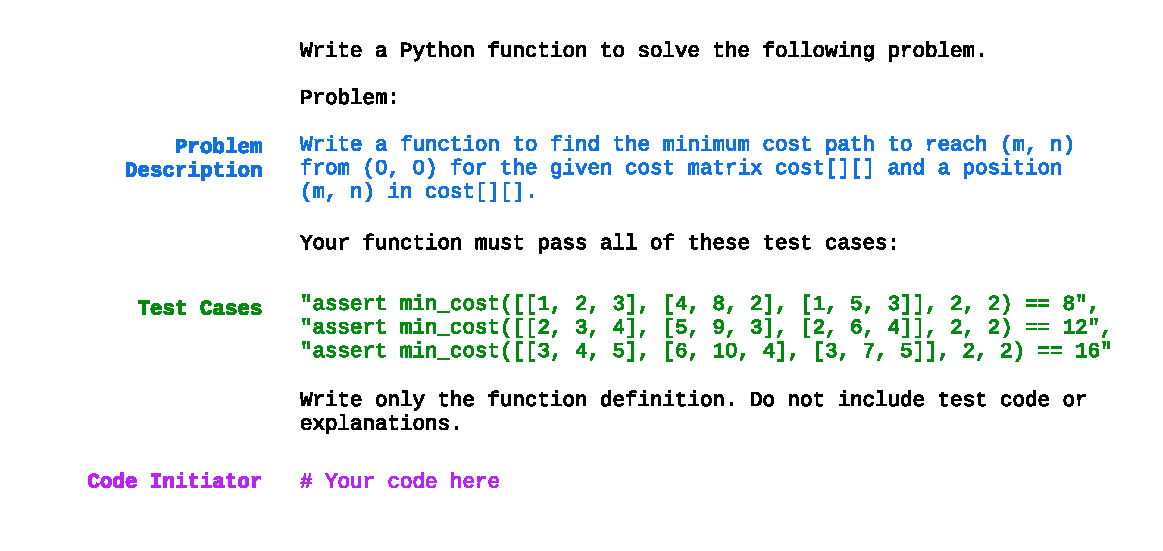
\includegraphics[width=1\linewidth]{figures/template.pdf}
    \caption{Standardized prompt template containing three components: problem description, test cases, and code initiator.}
    \label{fig:template}
\end{figure}

The template contains three essential components: the problem description provides the fundamental problem statement, test cases demonstrate expected input-output behavior with function signatures, and the code initiator ensures proper code generation from the base model. Context annotations clarify structure and purpose, ensuring consistent formatting while making the template's organization explicit for both human readers and the language model.

\textbf{Capture Stage}: During model inference, we capture residual stream activations at the final token position, providing the neural representations that will be decomposed through SAEs.

\textbf{Generate Stage}: Google's Gemma 2 language model with 2 billion parameters (\texttt{google/gemma-2-2b}) \citep{team2024gemma} generates code solutions. Temperature is set to 0 for deterministic, reproducible outputs that focus on the model's base behavior in code generation tasks.

\textbf{Evaluate Stage}: Each generated code solution is evaluated against MBPP test cases using pass@1 criterion. Solutions passing all test cases are classified as correct, while any failures (compilation errors, runtime exceptions, or incorrect outputs) result in incorrect classification.

\textbf{Decompose Stage}: The labeled samples and their corresponding activations undergo Sparse Autoencoder (SAE) decomposition using pre-trained models from GemmaScope. This stage transforms the raw neural activations into interpretable latent representations that can reveal program validity awareness patterns.

We employ the JumpReLU SAE architecture, which projects model representations $\mathbf{x} \in \mathbb{R}^d$ into a larger dimensional space $a(\mathbf{x}) \in \mathbb{R}^{d_{\text{SAE}}}$ to enable more granular analysis of neural activations. The encoding process applies a linear transformation followed by a JumpReLU activation function:

\begin{equation}
    a(\mathbf{x})=\text{JumpReLU}_{\theta}(\mathbf{xW}_{\text{enc}}+\mathbf{b}_{\text{enc}})
\end{equation}

where JumpReLU implements a threshold activation defined as:

\begin{equation}
    \text{JumpReLU}_\theta(\mathbf{x}) = \mathbf{x} \odot H(\mathbf{x} - \theta)
\end{equation}

Here, $H$ represents the Heaviside step function, and $\theta$ is a learnable threshold vector. The decoder reconstructs the original representation through:

\begin{equation}
    \text{SAE}(\mathbf{x})=a(\mathbf{x})\mathbf{W}_{\text{dec}}+\mathbf{b}_{\text{dec}}
\end{equation}

The autoencoder training minimizes a combined loss function that balances reconstruction accuracy with sparsity:

\begin{equation}
    \mathcal{L}(\mathbf{x}) = \underbrace{\|\mathbf{x} - \text{SAE}(\mathbf{x})\|_2^2}_{\mathcal{L}_{\text{reconstruction}}} + \underbrace{\lambda \|a(\mathbf{x})\|_0}_{\mathcal{L}_{\text{sparsity}}}
\end{equation}

This decomposition addresses the superposition problem in neural networks, where multiple features are entangled within individual neurons. By expanding the captured activations into a higher-dimensional sparse space, the SAE disentangles these overlapping representations, enabling cleaner identification of program validity awareness (PVA) latent directions with reduced interference from other linguistic and computational features. The resulting sparse activations are then analyzed using the separation score methodology detailed in the SAE Analysis section.

\subsection{Calendar of Activities}

Table \ref{tab:timetableactivities} shows a Gantt chart of the activities. Each bullet represents approximately one week's worth of activity.

\begin{table}[!ht]
\resizebox{\linewidth}{!}{
  \centering
  \begin{tabular}{l|c|c|c|c|c|c|c|c|c}
        \toprule
        &  \multicolumn{8}{c}{2025} \\
        \textbf{Activity} & \textbf{Jan} & \textbf{Feb} & \textbf{Mar} & \textbf{Apr} & \textbf{May} & \textbf{Jun} & \textbf{Jul} & \textbf{Aug}  \\
        \midrule
        Dataset Building & & & & **** & **** & & &  \\
        \midrule
        SAE Activation Analysis & & & & & **** & **** & &  \\
        \midrule
        Statistical Analysis & & & & & & **** & **** &  \\
        \midrule
        Steering Analysis & & & & & & & **** & **** \\
        \midrule
        Documentation & **** & **** & **** & **** & **** & **** & **** & **** \\
        \bottomrule
  \end{tabular}
}
  \caption{Gantt Chart of Activities}
  \label{tab:timetableactivities}
\end{table}

% \section{Engines}

% To produce a PDF file, pdf\LaTeX{} is strongly recommended (over original \LaTeX{} plus dvips+ps2pdf or dvipdf).
% The style file \texttt{acl.sty} can also be used with
% lua\LaTeX{} and
% Xe\LaTeX{}, which are especially suitable for text in non-Latin scripts.
% The file \texttt{acl\_lualatex.tex} in this repository provides
% an example of how to use \texttt{acl.sty} with either
% lua\LaTeX{} or
% Xe\LaTeX{}.

% \section{Preamble}

% The first line of the file must be
% \begin{quote}
% \begin{verbatim}
% \documentclass[11pt]{article}
% \end{verbatim}
% \end{quote}

% To load the style file in the review version:
% \begin{quote}
% \begin{verbatim}
% \usepackage[review]{acl}
% \end{verbatim}
% \end{quote}
% For the final version, omit the \verb|review| option:
% \begin{quote}
% \begin{verbatim}
% \usepackage{acl}
% \end{verbatim}
% \end{quote}

% To use Times Roman, put the following in the preamble:
% \begin{quote}
% \begin{verbatim}
% \usepackage{times}
% \end{verbatim}
% \end{quote}
% (Alternatives like txfonts or newtx are also acceptable.)

% Please see the \LaTeX{} source of this document for comments on other packages that may be useful.

% Set the title and author using \verb|\title| and \verb|\author|. Within the author list, format multiple authors using \verb|\and| and \verb|\And| and \verb|\AND|; please see the \LaTeX{} source for examples.

% By default, the box containing the title and author names is set to the minimum of 5 cm. If you need more space, include the following in the preamble:
% \begin{quote}
% \begin{verbatim}
% \setlength\titlebox{<dim>}
% \end{verbatim}
% \end{quote}
% where \verb|<dim>| is replaced with a length. Do not set this length smaller than 5 cm.

% \section{Document Body}

% \subsection{Footnotes}

% Footnotes are inserted with the \verb|\footnote| command.\footnote{This is a footnote.}

% \subsection{Tables and figures}

% See Table~\ref{tab:accents} for an example of a table and its caption.
% \textbf{Do not override the default caption sizes.}

% \begin{table}
%   \centering
%   \begin{tabular}{lc}
%     \hline
%     \textbf{Command} & \textbf{Output} \\
%     \hline
%     \verb|{\"a}|     & {\"a}           \\
%     \verb|{\^e}|     & {\^e}           \\
%     \verb|{\`i}|     & {\`i}           \\
%     \verb|{\.I}|     & {\.I}           \\
%     \verb|{\o}|      & {\o}            \\
%     \verb|{\'u}|     & {\'u}           \\
%     \verb|{\aa}|     & {\aa}           \\\hline
%   \end{tabular}
%   \begin{tabular}{lc}
%     \hline
%     \textbf{Command} & \textbf{Output} \\
%     \hline
%     \verb|{\c c}|    & {\c c}          \\
%     \verb|{\u g}|    & {\u g}          \\
%     \verb|{\l}|      & {\l}            \\
%     \verb|{\~n}|     & {\~n}           \\
%     \verb|{\H o}|    & {\H o}          \\
%     \verb|{\v r}|    & {\v r}          \\
%     \verb|{\ss}|     & {\ss}           \\
%     \hline
%   \end{tabular}
%   \caption{Example commands for accented characters, to be used in, \emph{e.g.}, Bib\TeX{} entries.}
%   \label{tab:accents}
% \end{table}

% As much as possible, fonts in figures should conform
% to the document fonts. See Figure~\ref{fig:experiments} for an example of a figure and its caption.

% Using the \verb|graphicx| package graphics files can be included within figure
% environment at an appropriate point within the text.
% The \verb|graphicx| package supports various optional arguments to control the
% appearance of the figure.
% You must include it explicitly in the \LaTeX{} preamble (after the
% \verb|\documentclass| declaration and before \verb|\begin{document}|) using
% \verb|\usepackage{graphicx}|.

% \begin{figure}[t]
%   \includegraphics[width=\columnwidth]{example-image-golden}
%   \caption{A figure with a caption that runs for more than one line.
%     Example image is usually available through the \texttt{mwe} package
%     without even mentioning it in the preamble.}
%   \label{fig:experiments}
% \end{figure}

% \begin{figure*}[t]
%   \includegraphics[width=0.48\linewidth]{example-image-a} \hfill
%   \includegraphics[width=0.48\linewidth]{example-image-b}
%   \caption {A minimal working example to demonstrate how to place
%     two images side-by-side.}
% \end{figure*}

% \subsection{Hyperlinks}

% Users of older versions of \LaTeX{} may encounter the following error during compilation:
% \begin{quote}
% \verb|\pdfendlink| ended up in different nesting level than \verb|\pdfstartlink|.
% \end{quote}
% This happens when pdf\LaTeX{} is used and a citation splits across a page boundary. The best way to fix this is to upgrade \LaTeX{} to 2018-12-01 or later.

% \subsection{Citations}

% \begin{table*}
%   \centering
%   \begin{tabular}{lll}
%     \hline
%     \textbf{Output}           & \textbf{natbib command} & \textbf{ACL only command} \\
%     \hline
%     \citep{Gusfield:97}       & \verb|\citep|           &                           \\
%     \citetlp{Gusfield:97}     & \verb|\citetlp|         &                           \\
%     \citet{Gusfield:97}       & \verb|\citet|           &                           \\
%     \citeyearpar{Gusfield:97} & \verb|\citeyearpar|     &                           \\
%     \citeposs{Gusfield:97}    &                         & \verb|\citeposs|          \\
%     \hline
%   \end{tabular}
%   \caption{\label{citation-guide}
%     Citation commands supported by the style file.
%     The style is based on the natbib package and supports all natbib citation commands.
%     It also supports commands defined in previous ACL style files for compatibility.
%   }
% \end{table*}

% Table~\ref{citation-guide} shows the syntax supported by the style files.
% We encourage you to use the natbib styles.
% You can use the command \verb|\citet| (cite in text) to get ``author (year)'' citations, like this citation to a paper by \citet{Gusfield:97}.
% You can use the command \verb|\citep| (cite in parentheses) to get ``(author, year)'' citations \citep{Gusfield:97}.
% You can use the command \verb|\citetlp| (alternative cite without parentheses) to get ``author, year'' citations, which is useful for using citations within parentheses (e.g. \citetlp{Gusfield:97}).

% A possessive citation can be made with the command \verb|\citeposs|.
% This is not a standard natbib command, so it is generally not compatible
% with other style files.

% \subsection{References}

% \nocite{Ando2005,andrew2007scalable,rasooli-tetrault-2015}

% The \LaTeX{} and Bib\TeX{} style files provided roughly follow the American Psychological Association format.
% If your own bib file is named \texttt{custom.bib}, then placing the following before any appendices in your \LaTeX{} file will generate the references section for you:
% \begin{quote}
% \begin{verbatim}
% \bibliography{custom}
% \end{verbatim}
% \end{quote}

% You can obtain the complete ACL Anthology as a Bib\TeX{} file from \url{https://aclweb.org/anthology/anthology.bib.gz}.
% To include both the Anthology and your own .bib file, use the following instead of the above.
% \begin{quote}
% \begin{verbatim}
% \bibliography{anthology,custom}
% \end{verbatim}
% \end{quote}

% Please see Section~\ref{sec:bibtex} for information on preparing Bib\TeX{} files.

% \subsection{Equations}

% An example equation is shown below:
% \begin{equation}
%   \label{eq:example}
%   A = \pi r^2
% \end{equation}

% Labels for equation numbers, sections, subsections, figures and tables
% are all defined with the \verb|\label{label}| command and cross references
% to them are made with the \verb|\ref{label}| command.

% This an example cross-reference to Equation~\ref{eq:example}.

% \subsection{Appendices}

% Use \verb|\appendix| before any appendix section to switch the section numbering over to letters. See Appendix~\ref{sec:appendix} for an example.

% \section{Bib\TeX{} Files}
% \label{sec:bibtex}

% Unicode cannot be used in Bib\TeX{} entries, and some ways of typing special characters can disrupt Bib\TeX's alphabetization. The recommended way of typing special characters is shown in Table~\ref{tab:accents}.

% Please ensure that Bib\TeX{} records contain DOIs or URLs when possible, and for all the ACL materials that you reference.
% Use the \verb|doi| field for DOIs and the \verb|url| field for URLs.
% If a Bib\TeX{} entry has a URL or DOI field, the paper title in the references section will appear as a hyperlink to the paper, using the hyperref \LaTeX{} package.

% \section*{Limitations}

% This document does not cover the content requirements for ACL or any
% other specific venue.  Check the author instructions for
% information on
% maximum page lengths, the required ``Limitations'' section,
% and so on.

% \section*{Acknowledgments}

% This document has been adapted
% by Steven Bethard, Ryan Cotterell and Rui Yan
% from the instructions for earlier ACL and NAACL proceedings, including those for
% ACL 2019 by Douwe Kiela and Ivan Vuli\'{c},
% NAACL 2019 by Stephanie Lukin and Alla Roskovskaya,
% ACL 2018 by Shay Cohen, Kevin Gimpel, and Wei Lu,
% NAACL 2018 by Margaret Mitchell and Stephanie Lukin,
% Bib\TeX{} suggestions for (NA)ACL 2017/2018 from Jason Eisner,
% ACL 2017 by Dan Gildea and Min-Yen Kan,
% NAACL 2017 by Margaret Mitchell,
% ACL 2012 by Maggie Li and Michael White,
% ACL 2010 by Jing-Shin Chang and Philipp Koehn,
% ACL 2008 by Johanna D. Moore, Simone Teufel, James Allan, and Sadaoki Furui,
% ACL 2005 by Hwee Tou Ng and Kemal Oflazer,
% ACL 2002 by Eugene Charniak and Dekang Lin,
% and earlier ACL and EACL formats written by several people, including
% John Chen, Henry S. Thompson and Donald Walker.
% Additional elements were taken from the formatting instructions of the \emph{International Joint Conference on Artificial Intelligence} and the \emph{Conference on Computer Vision and Pattern Recognition}.

% Bibliography entries for the entire Anthology, followed by custom entries
%\bibliography{anthology,custom}
% Custom bibliography entries only
\bibliography{custom}

% \appendix

% \section{Example Appendix}
% \label{sec:appendix}

% This is an appendix.

\end{document}
